% ============================================================
%  CSE 396 — Assignment 3: Module Documentation
%  Autonomous Fire Detection and Suppression Rover
%  Group 2
% ============================================================

\documentclass[12pt,a4paper]{article}

% ── Core packages ────────────────────────────────────────────
\usepackage[utf8]{inputenc}
\usepackage[T1]{fontenc}
\usepackage{lmodern}
\usepackage{microtype}
\usepackage[a4paper, top=2.5cm, bottom=2.5cm, left=2.5cm, right=2.5cm]{geometry}

% ── Layout ───────────────────────────────────────────────────
\usepackage{setspace}
\usepackage{parskip}
\usepackage{enumitem}
\usepackage{needspace}
\usepackage{placeins}

% ── Tables ───────────────────────────────────────────────────
\usepackage{array}
\usepackage{longtable}
\usepackage{booktabs}
\usepackage{tabularx}

% ── Code listings ────────────────────────────────────────────
\usepackage{listings}
\usepackage{mdframed}

% ── Graphics & links ─────────────────────────────────────────
\usepackage{graphicx}
\usepackage{float}
\usepackage[table]{xcolor}
\usepackage{hyperref}

% ── Section / header formatting ──────────────────────────────
\usepackage{titlesec}
\usepackage{fancyhdr}
\usepackage{amsmath}
\usepackage{caption}

% ════════════════════════════════════════════════════════════
%  COLOUR PALETTE  (shared across all modules)
% ════════════════════════════════════════════════════════════
\definecolor{accent}{HTML}{1a3c6e}       % primary accent blue
\definecolor{lightbg}{HTML}{e8eef7}      % table row alt background
\definecolor{codebg}{HTML}{f0f4f8}       % code listing background
\definecolor{tablegray}{HTML}{aaaaaa}    % rule colour
\definecolor{warnbg}{HTML}{FFF3CD}       % warning box background
\definecolor{warnborder}{HTML}{C47A00}   % warning box border
\definecolor{notebg}{HTML}{EAF7EA}       % note box background
\definecolor{noteborder}{HTML}{2E7D32}   % note box border
\definecolor{textgray}{HTML}{444444}     % subdued text

% ════════════════════════════════════════════════════════════
%  HYPERREF
% ════════════════════════════════════════════════════════════
\hypersetup{
    colorlinks=true,
    linkcolor=accent,
    urlcolor=accent,
    pdftitle={CSE 396 -- Assignment 3: Module Documentation},
    pdfauthor={CSE 396 Group 2},
    bookmarksnumbered=true
}

% ════════════════════════════════════════════════════════════
%  SECTION FORMATTING
% ════════════════════════════════════════════════════════════
\titleformat{\section}
  {\large\bfseries\color{accent}}
  {\thesection.}{0.5em}{}
  [\vspace{-0.3em}{\color{lightbg}\rule{\linewidth}{1pt}}]

\titleformat{\subsection}
  {\normalsize\bfseries\color{accent}}
  {\thesubsection.}{0.5em}{}

\titleformat{\subsubsection}
  {\small\bfseries}
  {\thesubsubsection.}{0.5em}{}

\titlespacing{\section}{0pt}{20pt}{8pt}
\titlespacing{\subsection}{0pt}{12pt}{4pt}
\titlespacing{\subsubsection}{0pt}{8pt}{3pt}

% ════════════════════════════════════════════════════════════
%  COLUMN TYPES
% ════════════════════════════════════════════════════════════
\newcolumntype{L}[1]{>{\raggedright\arraybackslash}p{#1}}
\newcolumntype{C}[1]{>{\centering\arraybackslash}p{#1}}
\arrayrulecolor{tablegray}

% ════════════════════════════════════════════════════════════
%  TABLE HEADER HELPERS
% ════════════════════════════════════════════════════════════
\newcommand{\theadtext}[1]{\textcolor{white}{\textbf{#1}}}

% ════════════════════════════════════════════════════════════
%  CODE LISTING STYLE
% ════════════════════════════════════════════════════════════
\lstset{
    language=C,
    backgroundcolor=\color{codebg},
    basicstyle=\footnotesize\ttfamily,
    keywordstyle=\color{accent}\bfseries,
    commentstyle=\color{textgray}\itshape,
    stringstyle=\color{accent!70!black},
    numberstyle=\tiny\color{tablegray},
    numbers=left,
    numbersep=8pt,
    breaklines=true,
    frame=single,
    framerule=0.4pt,
    rulecolor=\color{tablegray!60},
    tabsize=4,
    showstringspaces=false,
    captionpos=b,
    aboveskip=6pt,
    belowskip=8pt,
    xleftmargin=8pt,
    xrightmargin=8pt,
    morekeywords={uint8_t,uint16_t,uint32_t,int8_t,int16_t,int32_t,bool,true,false}
}

% ════════════════════════════════════════════════════════════
%  CALLOUT BOXES
% ════════════════════════════════════════════════════════════
\newmdenv[backgroundcolor=warnbg, linecolor=warnborder, linewidth=1.2pt,
  innerleftmargin=10pt, innerrightmargin=10pt,
  innertopmargin=6pt, innerbottommargin=6pt]{warnbox}

\newmdenv[backgroundcolor=notebg, linecolor=noteborder, linewidth=1.2pt,
  innerleftmargin=10pt, innerrightmargin=10pt,
  innertopmargin=6pt, innerbottommargin=6pt]{notebox}

% ════════════════════════════════════════════════════════════
%  INLINE MONOSPACE SHORTHAND
% ════════════════════════════════════════════════════════════
\newcommand{\fn}[1]{{\footnotesize\ttfamily #1}}

% ════════════════════════════════════════════════════════════
%  HEADER / FOOTER
% ════════════════════════════════════════════════════════════
\pagestyle{fancy}
\fancyhf{}
\fancyhead[L]{\small\textcolor{textgray}{CSE 396 --- Group 2}}
\fancyhead[R]{\small\textcolor{textgray}{Module Documentation}}
\fancyfoot[C]{\thepage}
\renewcommand{\headrulewidth}{0.4pt}

% ════════════════════════════════════════════════════════════
%  GLOBAL SPACING
% ════════════════════════════════════════════════════════════
\setstretch{1.15}
\setlength{\parskip}{0.5em}
\setlength{\parindent}{0pt}

% ════════════════════════════════════════════════════════════
%  DOCUMENT START
% ════════════════════════════════════════════════════════════
\begin{document}

% ── COVER PAGE ───────────────────────────────────────────────
\begin{titlepage}
  \centering
  \vspace*{1.2cm}

  {\color{accent}\rule{\linewidth}{2pt}}
  \vspace{0.4cm}

  {\Huge\bfseries\color{accent} CSE 396}\\[0.3cm]
  {\Large\bfseries\color{accent} Computer Engineering Project}\\[0.6cm]

  {\color{textgray}\rule{\linewidth}{0.5pt}}
  \vspace{0.5cm}

  {\huge\bfseries Assignment 3}\\[0.2cm]
  {\LARGE Module Documentation}\\[0.3cm]
  {\large\textit{Autonomous Fire Detection and Suppression Rover}}\\[0.7cm]

  {\color{textgray}\rule{\linewidth}{0.5pt}}
  \vspace{0.7cm}

  {\large\bfseries Group 2}\\[0.4cm]

  \begin{tabular}{L{5cm} L{4cm} L{5cm}}
    \rowcolor{accent}
    \theadtext{Name} & \theadtext{Student ID} & \theadtext{Assigned Modules} \\
    \rowcolor{white}   Cemal G\"{U}M\"{U}\c{S}    & 210104004304 & MOD-01, MOD-03 \\
    \rowcolor{lightbg} Melih KAZANCI              & 230104004909 & MOD-01, MOD-03 \\
    \rowcolor{white}   Mehmet Alp ATAY            & 220104004020 & MOD-02, MOD-06 \\
    \rowcolor{lightbg} Adil Mert ERG\"{O}R\"{U}N  & 220104004048 & MOD-02, MOD-06 \\
    \rowcolor{white}   Ahmet Halil YAMLI          & 220104004957 & MOD-04, MOD-05 \\
    \rowcolor{lightbg} Derya UYSAL                & 220104004045 & MOD-04, MOD-05 \\
    \rowcolor{white}   Ay\c{s}e Feyza SERBEST     & 220104004052 & MOD-07, MOD-08 \\
    \rowcolor{lightbg} G\"{o}rkem UYSAL           & 230104004174 & MOD-07, MOD-08 \\
  \end{tabular}

  \vspace{0.8cm}
  {\large April 2026}

  \vfill
  {\color{accent}\rule{\linewidth}{2pt}}
\end{titlepage}

% ── TABLE OF CONTENTS ────────────────────────────────────────
\tableofcontents
\newpage

% ════════════════════════════════════════════════════════════
%  SYSTEM OVERVIEW
% ════════════════════════════════════════════════════════════
\section*{System Overview}
\addcontentsline{toc}{section}{System Overview}

The Autonomous Fire Detection and Suppression Rover is an embedded system designed
to autonomously detect, approach, and extinguish fires. It is built around eight
interconnected modules, each with clearly defined responsibilities and interfaces.

\begin{table}[H]
\centering\small
\begin{tabularx}{\textwidth}{L{1.6cm} L{5cm} X}
\toprule
\rowcolor{accent}
\theadtext{Module} & \theadtext{Name} & \theadtext{Role} \\
\midrule
\rowcolor{white}   MOD-01 & Flame Sensing Hardware      & Physical IR sensor acquisition \\
\rowcolor{lightbg} MOD-02 & Flame Detection Software    & Signal processing and direction estimation \\
\rowcolor{white}   MOD-03 & Locomotion Hardware         & Chassis, motors, and motor driver \\
\rowcolor{lightbg} MOD-04 & Motion Control Software     & High-level motion command translation \\
\rowcolor{white}   MOD-05 & Distance Sensing Software   & Ultrasonic obstacle detection \\
\rowcolor{lightbg} MOD-06 & Fire Suppression Hardware   & Relay-driven water pump control \\
\rowcolor{white}   MOD-07 & Autonomy Software           & Central FSM and mission decision logic \\
\rowcolor{lightbg} MOD-08 & Integration \& Test Module  & System-wide validation and simulation \\
\bottomrule
\end{tabularx}
\caption{System module summary}
\end{table}

The overall system structure and inter-module data flow are illustrated in Figure~\ref{fig:block-diagram}.

\begin{figure}[H]
    \centering
    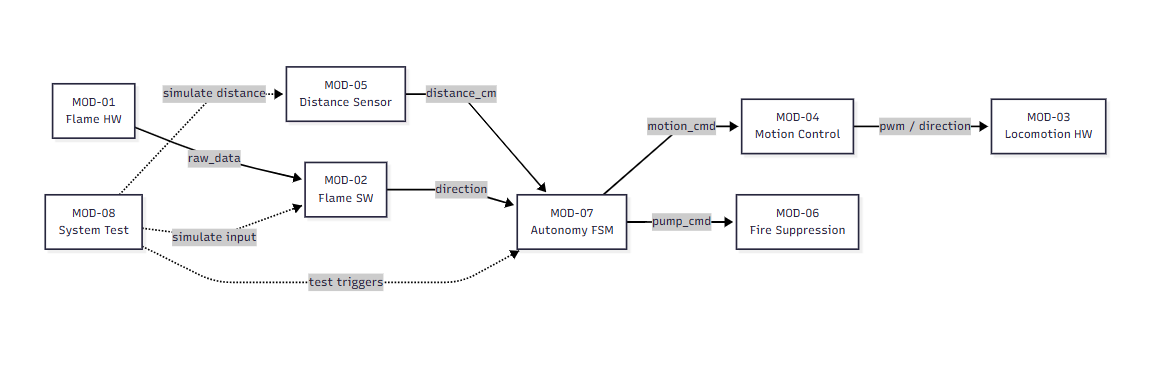
\includegraphics[width=0.95\linewidth]{diagram.png}
    \caption{System / module block diagram}
    \label{fig:block-diagram}
\end{figure}

\newpage

% ════════════════════════════════════════════════════════════
%  MOD-01 — FLAME SENSING HARDWARE
% ════════════════════════════════════════════════════════════
\section{MOD-01 --- Flame Sensing Hardware}

\subsection{Module Purpose}

MOD-01 is responsible for the physical detection of flame-related infrared signals
in the environment. Its main task is to acquire raw sensor information and transmit
this information to the software layer for further processing.

Within the rover architecture, this module forms the first stage of the fire
detection process. It does not make decisions by itself; instead, it acts as the
hardware source of flame intensity data.

\subsection{Main Responsibilities}

\begin{itemize}[leftmargin=1.5em]
  \item Mounting the flame sensors onto the rover body.
  \item Wiring the sensors to the microcontroller.
  \item Ensuring stable analog signal acquisition.
  \item Reducing noise and ambient light interference.
  \item Providing raw sensor data for software processing.
\end{itemize}

\subsection{Working Principle}

The flame sensors detect infrared radiation emitted by a flame source. Each sensor
produces an electrical output corresponding to the detected intensity. These outputs
are read by the microcontroller via its ADC channels.

By placing multiple flame sensors in different directions (left, center, and right),
the system can compare the measured intensity values and estimate the direction of
the flame. MOD-01 therefore provides the physical sensing basis for directional
flame localization.

\subsection{Inputs and Outputs}

\begin{table}[H]
\centering\small
\begin{tabularx}{\textwidth}{L{3cm} L{3cm} X}
\toprule
\rowcolor{accent}
\theadtext{Flow} & \theadtext{Signal} & \theadtext{Description} \\
\midrule
\rowcolor{white}   Input  & Infrared energy   & IR radiation emitted by flame source \\
\rowcolor{lightbg} Input  & Supply voltage    & Power for sensor electronics \\
\rowcolor{white}   Input  & Sensor orientation & Physical mounting direction \\
\rowcolor{lightbg} Output & Raw analog values & 10-bit ADC readings (left, center, right) \\
\rowcolor{white}   Output & Digital threshold & Optional digital HIGH/LOW per sensor \\
\bottomrule
\end{tabularx}
\caption{MOD-01 inputs and outputs}
\end{table}

\textbf{Output Destination:} Raw sensor values are sent to \textbf{MOD-02 (Flame Detection Software)} for filtering, thresholding, and direction estimation.

\subsection{Connection to Other Modules}

MOD-01 directly communicates with MOD-02 by supplying raw flame sensor values.
MOD-02 then processes this data and forwards flame-related information to the
autonomy layer. The processing chain is:

\begin{center}
\textbf{MOD-01 $\rightarrow$ MOD-02 $\rightarrow$ MOD-07}
\end{center}

This means that MOD-01 indirectly affects rover navigation and suppression
decisions, even though it does not control those modules directly.

\subsection{Technical Design Notes}

\begin{itemize}[leftmargin=1.5em]
  \item Sensor placement was selected to maximize field of view.
  \item Wiring was arranged to reduce electrical noise.
  \item Analog output was preferred because it provides richer intensity information than a digital threshold alone.
  \item Care was taken to reduce false readings caused by ambient light.
  \item Sensor orientation and spacing were adjusted to improve directional reliability.
\end{itemize}

\subsection{Known Limitations}

\begin{itemize}[leftmargin=1.5em]
  \item False positives caused by strong ambient light (e.g., sunlight or incandescent lamps).
  \item Sensitivity to reflective surfaces that scatter IR radiation.
  \item Unstable readings due to electrical noise on unshielded wiring.
  \item Incorrect direction estimation if sensor placement or spacing is suboptimal.
\end{itemize}

\subsection{Testing and Verification}

\begin{itemize}[leftmargin=1.5em]
  \item Checking whether each sensor produces a valid output signal.
  \item Comparing readings for left, center, and right flame positions.
  \item Testing under different ambient light conditions.
  \item Verifying successful data transfer to MOD-02.
\end{itemize}

\newpage

% ════════════════════════════════════════════════════════════
%  MOD-02 — FLAME DETECTION SOFTWARE
% ════════════════════════════════════════════════════════════
\section{MOD-02 --- Flame Detection Software}

\subsection{Module Overview}

MOD-02 is the software layer that reads raw ADC values from MOD-01 (Flame Sensing
Hardware) and produces structured, semantically meaningful flame detection results
consumed by the Autonomy FSM (MOD-07). It is the only module that knows the
\emph{meaning} of IR sensor readings: it applies thresholding, determines which
sensor is dominant, and assigns a directional label.

\begin{table}[H]
\centering\small
\begin{tabularx}{\textwidth}{L{2.8cm} L{3cm} X}
\toprule
\rowcolor{accent}
\theadtext{Direction} & \theadtext{Module} & \theadtext{Interface} \\
\midrule
\rowcolor{white}   Upstream (input)    & MOD-01 Flame HW & \fn{flame\_hw\_read\_raw(uint16\_t *buffer)} --- populates \fn{raw[3]} \\
\rowcolor{lightbg} Downstream (output) & MOD-07 Autonomy & \fn{flame\_data\_t} via \fn{flame\_read()} or callback \\
\bottomrule
\end{tabularx}
\caption{MOD-02 inter-module connections}
\end{table}

\textbf{Header file:} \fn{Header\ files/MOD\ 02/flame\_detection.h}

\subsection{Constants and Macros}

\begin{table}[H]
\centering\small
\begin{tabularx}{\textwidth}{L{5cm} L{2cm} X}
\toprule
\rowcolor{accent}
\theadtext{Macro} & \theadtext{Value} & \theadtext{Rationale} \\
\midrule
\rowcolor{white}   \fn{FLAME\_SENSOR\_COUNT}        & \fn{3}    & Three KY-026 IR sensors mounted left, center, right. Mirrors \fn{FLAME\_HW\_SENSOR\_COUNT} from MOD-01. \\
\rowcolor{lightbg} \fn{FLAME\_THRESHOLD}            & \fn{500}  & ADC reading (0--1023) above which a sensor is considered detecting flame. Mirrors \fn{FLAME\_HW\_THRESHOLD\_DEFAULT} from MOD-01; must be validated experimentally. \\
\rowcolor{white}   \fn{FLAME\_SAMPLE\_INTERVAL\_MS} & \fn{50}   & Sampling period in milliseconds (20~Hz). Balances responsiveness vs.\@ CPU load on the ESP32. \\
\rowcolor{lightbg} \fn{FLAME\_ADC\_MAX}             & \fn{1023} & Full-scale value of the 10-bit ADC on the ESP32. Used for normalization if needed. \\
\bottomrule
\end{tabularx}
\caption{MOD-02 constants and their rationale}
\end{table}

\subsection{Data Types}

\subsubsection{\fn{flame\_status\_t} --- Return / Error Codes}

\begin{table}[H]
\centering\small
\begin{tabularx}{\textwidth}{L{4.5cm} C{1cm} X}
\toprule
\rowcolor{accent}
\theadtext{Enumerator} & \theadtext{Value} & \theadtext{Meaning} \\
\midrule
\rowcolor{white}   \fn{FLAME\_OK}              & \fn{0}  & Operation completed successfully. \\
\rowcolor{lightbg} \fn{FLAME\_ERR\_INIT}       & \fn{-1} & Hardware initialisation failed. Module must not be used until successful re-init. \\
\rowcolor{white}   \fn{FLAME\_ERR\_NO\_SENSOR} & \fn{-2} & One or more sensors not responding (ADC returns 0 or 1023 persistently). \\
\rowcolor{lightbg} \fn{FLAME\_ERR\_TIMEOUT}    & \fn{-3} & No new sample produced yet (first call before first sampling cycle). \\
\bottomrule
\end{tabularx}
\caption{\fn{flame\_status\_t} enumerator definitions}
\end{table}

\subsubsection{\fn{flame\_direction\_t} --- Detected Flame Direction}

\begin{table}[H]
\centering\small
\begin{tabularx}{\textwidth}{L{4cm} C{1cm} X}
\toprule
\rowcolor{accent}
\theadtext{Enumerator} & \theadtext{Value} & \theadtext{Meaning} \\
\midrule
\rowcolor{white}   \fn{FLAME\_DIR\_NONE}   & \fn{0} & No sensor exceeded threshold; no flame detected. \\
\rowcolor{lightbg} \fn{FLAME\_DIR\_LEFT}   & \fn{1} & Left sensor (\fn{raw[0]}) has the highest reading above threshold. \\
\rowcolor{white}   \fn{FLAME\_DIR\_CENTER} & \fn{2} & Center sensor (\fn{raw[1]}) has the highest reading. \\
\rowcolor{lightbg} \fn{FLAME\_DIR\_RIGHT}  & \fn{3} & Right sensor (\fn{raw[2]}) has the highest reading. \\
\bottomrule
\end{tabularx}
\caption{\fn{flame\_direction\_t} enumerator definitions}
\end{table}


\subsubsection{\fn{flame\_data\_t} --- Aggregated Sensor Reading}

This is the primary struct shared with MOD-07. It is populated on every sampling cycle.

\begin{table}[H]
\centering\small
\begin{tabularx}{\textwidth}{L{3.8cm} L{2.5cm} L{2cm} X}
\toprule
\rowcolor{accent}
\theadtext{Field} & \theadtext{Type} & \theadtext{Range} & \theadtext{Description} \\
\midrule
\rowcolor{white}   \fn{raw[FLAME\_SENSOR\_COUNT]} & \fn{uint16\_t[3]} & 0--1023       & Raw 10-bit ADC readings. Index 0 = left, 1 = center, 2 = right. \\
\rowcolor{lightbg} \fn{max\_intensity}  & \fn{uint16\_t}       & 0--1023       & Highest value among \fn{raw[0..2]}. Proxy for flame proximity. \\
\rowcolor{white}   \fn{detected}        & \fn{uint8\_t}        & 0 or 1        & Non-zero if \fn{max\_intensity > FLAME\_THRESHOLD}. \\
\rowcolor{lightbg} \fn{direction}       & \fn{flame\_direction\_t} & enum      & Dominant direction. Only meaningful when \fn{detected == 1}. \\
\rowcolor{white}   \fn{timestamp\_ms}   & \fn{uint32\_t}       & ms since boot & Time of reading via \fn{millis()}. MOD-07 should reject data older than 100~ms. \\
\bottomrule
\end{tabularx}
\caption{\fn{flame\_data\_t} field descriptions}
\end{table}

\subsubsection{\fn{flame\_cb\_t} --- Sampling Callback}

\begin{lstlisting}[caption={Callback typedef}]
typedef void (*flame_cb_t)(const flame_data_t *data);
\end{lstlisting}

Invoked \emph{synchronously} at the end of each 50~ms sampling cycle with a
read-only pointer to the freshly populated \fn{flame\_data\_t}.


\subsection{Public API}

\subsubsection{\fn{flame\_init()}}

\begin{lstlisting}[caption={Signature}]
flame_status_t flame_init(void);
\end{lstlisting}

\begin{table}[H]\centering\small
\begin{tabularx}{\textwidth}{L{3cm} X}
\toprule
\rowcolor{accent}\theadtext{Attribute} & \theadtext{Detail} \\
\midrule
\rowcolor{white}   Pre-condition  & None. Safe to call at any point, including after a failed init. \\
\rowcolor{lightbg} Post-condition & On \fn{FLAME\_OK}: ADC pins configured, module ready. On error: state undefined; retry. \\
\rowcolor{white}   Calls          & \fn{flame\_hw\_init()} from MOD-01. \\
\rowcolor{lightbg} Returns        & \fn{FLAME\_OK} or \fn{FLAME\_ERR\_INIT}. \\
\rowcolor{white}   Side effects   & Configures ESP32 ADC channels. Does \textbf{not} start sampling. \\
\bottomrule
\end{tabularx}
\end{table}

\subsubsection{\fn{flame\_start()}}

\begin{lstlisting}[caption={Signature}]
flame_status_t flame_start(flame_cb_t cb);
\end{lstlisting}

\begin{table}[H]\centering\small
\begin{tabularx}{\textwidth}{L{3cm} X}
\toprule
\rowcolor{accent}\theadtext{Attribute} & \theadtext{Detail} \\
\midrule
\rowcolor{white}   Pre-condition  & \fn{flame\_init()} returned \fn{FLAME\_OK}. \\
\rowcolor{lightbg} Parameters     & \fn{cb} -- callback per sample; pass \fn{NULL} to use pull model only. \\
\rowcolor{white}   Post-condition & 20~Hz sampling begins. Each cycle: reads ADC, computes direction, updates buffer, invokes \fn{cb} if set. \\
\rowcolor{lightbg} Returns        & \fn{FLAME\_OK}. \\
\rowcolor{white}   Side effects   & Starts repeating timer; consumes CPU proportional to sampling rate. \\
\bottomrule
\end{tabularx}
\end{table}

\subsubsection{\fn{flame\_read()}}

\begin{lstlisting}[caption={Signature}]
flame_status_t flame_read(flame_data_t *out);
\end{lstlisting}

\begin{table}[H]\centering\small
\begin{tabularx}{\textwidth}{L{3cm} X}
\toprule
\rowcolor{accent}\theadtext{Attribute} & \theadtext{Detail} \\
\midrule
\rowcolor{white}   Pre-condition  & \fn{flame\_start()} called. \fn{out} points to valid memory. \\
\rowcolor{lightbg} Post-condition & \fn{*out} populated with the latest sample. \\
\rowcolor{white}   Returns        & \fn{FLAME\_OK} if data available; \fn{FLAME\_ERR\_TIMEOUT} if no sample yet. \\
\rowcolor{lightbg} Thread safety  & Safe to call from main loop while sampling runs. \\
\bottomrule
\end{tabularx}
\end{table}

\subsubsection{\fn{flame\_get\_direction()}}

\begin{lstlisting}[caption={Signature}]
flame_direction_t flame_get_direction(void);
\end{lstlisting}

\begin{table}[H]\centering\small
\begin{tabularx}{\textwidth}{L{3cm} X}
\toprule
\rowcolor{accent}\theadtext{Attribute} & \theadtext{Detail} \\
\midrule
\rowcolor{white}   Pre-condition  & At least one sampling cycle completed. \\
\rowcolor{lightbg} Returns        & Current dominant direction. Returns \fn{FLAME\_DIR\_NONE} if no sample yet. \\
\rowcolor{white}   Use case       & Lightweight FSM polling when only direction is needed. \\
\bottomrule
\end{tabularx}
\end{table}

\subsubsection{\fn{flame\_stop()}}

\begin{lstlisting}[caption={Signature}]
void flame_stop(void);
\end{lstlisting}

\begin{table}[H]\centering\small
\begin{tabularx}{\textwidth}{L{3cm} X}
\toprule
\rowcolor{accent}\theadtext{Attribute} & \theadtext{Detail} \\
\midrule
\rowcolor{white}   Pre-condition  & None. Safe to call even if not started. \\
\rowcolor{lightbg} Post-condition & Sampling halted. Last sample retained in buffer. \\
\rowcolor{white}   Side effects   & Pending callback cancelled. Call \fn{flame\_init()} + \fn{flame\_start()} to resume. \\
\bottomrule
\end{tabularx}
\end{table}

\subsection{Timing and Sampling Behaviour}

\begin{table}[H]\centering\small
\begin{tabularx}{\textwidth}{L{5cm} X}
\toprule
\rowcolor{accent}\theadtext{Parameter} & \theadtext{Value / Notes} \\
\midrule
\rowcolor{white}   Sampling interval    & 50~ms (20~Hz) --- \fn{FLAME\_SAMPLE\_INTERVAL\_MS} \\
\rowcolor{lightbg} ADC conversion time  & $\approx$5~$\mu$s per channel; three channels $\approx$15~$\mu$s total. \\
\rowcolor{white}   Callback deadline    & Must return within $\ll$50~ms to avoid missing the next cycle. \\
\rowcolor{lightbg} Data staleness limit & MOD-07 should reject \fn{flame\_data\_t} with \fn{timestamp\_ms} older than 100~ms. \\
\bottomrule
\end{tabularx}
\caption{MOD-02 timing parameters}
\end{table}

\subsection{Inter-Module Protocol: MOD-01 $\rightarrow$ MOD-02 $\rightarrow$ MOD-07}

\begin{enumerate}[leftmargin=*, label=\textbf{Step \arabic*.}]
  \item \textbf{Hardware read.} MOD-02 calls \fn{flame\_hw\_read\_raw(raw)} (MOD-01). Three 10-bit ADC values written into \fn{raw[0..2]}: left, center, right.
  \item \textbf{Threshold check.} For each \fn{raw[i]}, compare to \fn{FLAME\_THRESHOLD = 500}.
  \item \textbf{Max intensity.} \fn{max\_intensity = max(raw[0], raw[1], raw[2])}.
  \item \textbf{Detection flag.} \fn{detected = (max\_intensity > FLAME\_THRESHOLD) ? 1 : 0}.
  \item \textbf{Direction.} Index with highest \fn{raw[i]} exceeding threshold $\rightarrow$ direction enum. If none exceed threshold $\rightarrow$ \fn{FLAME\_DIR\_NONE}.
  \item \textbf{Timestamp.} \fn{timestamp\_ms = millis()}.
  \item \textbf{Publish.} Buffer updated. Callback invoked (if registered). MOD-07 calls \fn{flame\_read()} or reads callback argument.
\end{enumerate}

\subsection{Error Handling Guide}

\begin{table}[H]\centering\small
\begin{tabularx}{\textwidth}{L{4.5cm} X}
\toprule
\rowcolor{accent}\theadtext{Error Code} & \theadtext{Recommended Action} \\
\midrule
\rowcolor{white}   \fn{FLAME\_ERR\_INIT}       & Wait 100~ms, retry \fn{flame\_init()}. After 3 consecutive failures, halt and signal MOD-08. \\
\rowcolor{lightbg} \fn{FLAME\_ERR\_NO\_SENSOR} & Check ADC wiring. Treat as hardware fault; do not continue with faulty sensor. \\
\rowcolor{white}   \fn{FLAME\_ERR\_TIMEOUT}    & Retry after \fn{FLAME\_SAMPLE\_INTERVAL\_MS + 10}~ms. If persistent, call \fn{flame\_stop()} then \fn{flame\_start()}. \\
\bottomrule
\end{tabularx}
\caption{MOD-02 error handling recommendations}
\end{table}


\subsection{Known Limitations and TODOs}

\begin{itemize}[leftmargin=1.5em]
  \item \textbf{Ambient light interference.} Strong sunlight or incandescent lamps generate IR indistinguishable from flame by the KY-026. Shielded housings are recommended.
  \item \textbf{Single-axis detection only.} Left/center/right only; no elevation angle.
  \item \textbf{Winner-takes-all direction.} A weighted average of all \fn{raw[i]} would provide finer directional precision.
  \item \textbf{Callback thread safety.} If FreeRTOS tasks are used, a mutex must protect the shared buffer.
  \item \textbf{TODO:} Moving-average filter over last $N$ samples before threshold comparison.
  \item \textbf{TODO:} Add \fn{FLAME\_ERR\_STALE} when \fn{timestamp\_ms} has not updated within $2 \times$ \fn{FLAME\_SAMPLE\_INTERVAL\_MS}.
\end{itemize}

\newpage

% ════════════════════════════════════════════════════════════
%  MOD-03 — LOCOMOTION HARDWARE
% ════════════════════════════════════════════════════════════
\section{MOD-03 --- Locomotion Hardware}

\subsection{Module Purpose}

MOD-03 is responsible for the physical movement infrastructure of the rover. This
includes the motor driver, DC motors, wheel assembly, and the electrical connections
required for motion.

This module is the hardware execution layer of the movement subsystem. It receives
low-level motion control signals and converts them into real motor actuation.

\subsection{Main Responsibilities}

\begin{itemize}[leftmargin=1.5em]
  \item Chassis assembly and structural mounting.
  \item Motor mounting and alignment.
  \item Motor driver wiring (L298N connections).
  \item Battery and power connection setup.
  \item Enabling directional motor control.
  \item Enabling PWM-based speed control.
\end{itemize}

\subsection{Working Principle}

The locomotion subsystem uses a \textbf{differential drive} mechanism. The motor
driver receives control inputs from the microcontroller, including direction and
PWM-based speed commands. These control signals are translated into motor actuation
for the left and right wheels.

By changing the speed and direction of each motor independently, the rover can move
forward, backward, turn left, turn right, or stop. MOD-03 therefore provides the
physical actuation required for navigation.

\subsection{Inputs and Outputs}

\begin{table}[H]
\centering\small
\begin{tabularx}{\textwidth}{L{3cm} L{3cm} X}
\toprule
\rowcolor{accent}
\theadtext{Flow} & \theadtext{Signal} & \theadtext{Description} \\
\midrule
\rowcolor{white}   Input  & PWM signals     & Speed control signals from MOD-04 \\
\rowcolor{lightbg} Input  & Direction lines & Motor direction control signals from MOD-04 \\
\rowcolor{white}   Input  & Battery power   & Supply voltage for motors and driver \\
\rowcolor{lightbg} Output & Wheel rotation  & Physical rotation of left and right wheels \\
\rowcolor{white}   Output & Rover movement  & Resulting rover displacement in the physical environment \\
\bottomrule
\end{tabularx}
\caption{MOD-03 inputs and outputs}
\end{table}

\textbf{Input Source:} Low-level motion signals are received from \textbf{MOD-04 (Motion Control Software)}.

\subsection{Connection to Other Modules}

MOD-03 receives actuation signals from MOD-04, which converts higher-level motion
commands into motor-specific low-level outputs. The control chain is:

\begin{center}
\textbf{MOD-07 $\rightarrow$ MOD-04 $\rightarrow$ MOD-03}
\end{center}

In this structure: MOD-07 decides what the rover should do, MOD-04 translates this
decision into motor commands, and MOD-03 physically executes the movement.

\subsection{Technical Design Notes}

\begin{itemize}[leftmargin=1.5em]
  \item Differential drive was selected because it is simple and suitable for indoor rover navigation.
  \item The L298N driver is used to control two DC motors independently.
  \item PWM control allows adjustable speed instead of only ON/OFF operation.
  \item Wheel alignment and chassis stability were considered during assembly.
\end{itemize}

\subsection{Known Limitations}

\begin{itemize}[leftmargin=1.5em]
  \item Wheel slipping during sudden starts without acceleration ramping.
  \item Imbalance between left and right motors due to manufacturing variation.
  \item Battery voltage drop reducing motor performance over time.
  \item Chassis vibration affecting movement stability on rough surfaces.
  \item Motor driver inefficiency or overheating under sustained load.
\end{itemize}

\subsection{Testing and Verification}

\begin{itemize}[leftmargin=1.5em]
  \item Checking forward and backward motion integrity.
  \item Checking left and right turning behavior.
  \item Verifying stop response latency.
  \item Verifying PWM-based speed adjustment across the 0--255 range.
  \item Testing motor direction consistency.
  \item Checking movement stability under battery power at various charge levels.
\end{itemize}

\newpage

% ════════════════════════════════════════════════════════════
%  MOD-04 — MOTION CONTROL SOFTWARE
% ════════════════════════════════════════════════════════════
\section{MOD-04 --- Motion Control Software}

\subsection{Module Overview}

MOD-04 is the software layer that converts high-level movement requests from MOD-07
into low-level differential drive commands executed by MOD-03 (Locomotion Hardware).
It abstracts direction and speed into PWM and GPIO signals.

\begin{table}[H]
\centering\small
\begin{tabularx}{\textwidth}{L{2.8cm} L{2.8cm} X}
\toprule
\rowcolor{accent}
\theadtext{Direction} & \theadtext{Module} & \theadtext{Interface} \\
\midrule
\rowcolor{white}   Upstream (input)    & MOD-07 Autonomy & \fn{motion\_cmd} (direction and speed) \\
\rowcolor{lightbg} Downstream (output) & MOD-03 Locomotion HW & PWM and direction control lines \\
\bottomrule
\end{tabularx}
\caption{MOD-04 inter-module connections}
\end{table}

\subsection{Constants and Macros}

\begin{table}[H]
\centering\small
\begin{tabularx}{\textwidth}{L{5.5cm} L{2.5cm} X}
\toprule
\rowcolor{accent}
\theadtext{Name} & \theadtext{Value} & \theadtext{Purpose} \\
\midrule
\rowcolor{white}   \fn{MOTION\_DEFAULT\_SPEED}    & \fn{150} & Default PWM speed value (0--255) for normal drive commands. \\
\rowcolor{lightbg} \fn{MOTION\_MIN\_THRESHOLD}    & \fn{LOCO\_HW\_MIN\_PWM} & Minimum effective PWM level to overcome wheel static friction. Aliases \fn{LOCO\_HW\_MIN\_PWM} (60) from MOD-03. \\
\bottomrule
\end{tabularx}
\caption{MOD-04 constants}
\end{table}

\subsection{Data Types}

\subsubsection{\fn{motion\_status\_t} --- Return / Error Codes}

\begin{table}[H]
\centering\small
\begin{tabularx}{\textwidth}{L{4.5cm} C{1cm} X}
\toprule
\rowcolor{accent}
\theadtext{Enumerator} & \theadtext{Value} & \theadtext{Meaning} \\
\midrule
\rowcolor{white}   \fn{MOTION\_OK}         & \fn{0}  & Operation completed successfully. \\
\rowcolor{lightbg} \fn{MOTION\_ERR\_DRIVER} & \fn{-1} & Motor driver communication or actuation failure. \\
\rowcolor{white}   \fn{MOTION\_ERR\_PARAM}  & \fn{-2} & Invalid speed or direction argument was provided. \\
\bottomrule
\end{tabularx}
\caption{\fn{motion\_status\_t} enumerator definitions}
\end{table}

\subsubsection{\fn{motion\_direction\_t} --- Direction Enumeration}

\begin{table}[H]
\centering\small
\begin{tabularx}{\textwidth}{L{5cm} X}
\toprule
\rowcolor{accent}
\theadtext{Enumerator} & \theadtext{Meaning} \\
\midrule
\rowcolor{white}   \fn{MOTION\_DIR\_STOP}     & Stop both motors immediately. \\
\rowcolor{lightbg} \fn{MOTION\_DIR\_FORWARD}  & Move rover forward. \\
\rowcolor{white}   \fn{MOTION\_DIR\_BACKWARD} & Move rover backward. \\
\rowcolor{lightbg} \fn{MOTION\_DIR\_LEFT}     & Perform differential left turn. \\
\rowcolor{white}   \fn{MOTION\_DIR\_RIGHT}    & Perform differential right turn. \\
\bottomrule
\end{tabularx}
\caption{\fn{motion\_direction\_t} enumerator definitions}
\end{table}

\subsection{Public API}

\begin{table}[H]
\centering\small
\begin{tabularx}{\textwidth}{L{5cm} L{4cm} L{2.5cm} X}
\toprule
\rowcolor{accent}
\theadtext{Function} & \theadtext{Parameters} & \theadtext{Return} & \theadtext{Description} \\
\midrule
\rowcolor{white}   \fn{motion\_init()}             & \fn{void} & \fn{motion\_status\_t} & Initializes motor pins and PWM channels. \\
\rowcolor{lightbg} \fn{motion\_drive()}            & \fn{motion\_direction\_t dir, uint8\_t speed} & \fn{motion\_status\_t} & Converts abstract direction and speed to low-level driver commands. \\
\rowcolor{white}   \fn{motion\_set\_differential()} & \fn{int16\_t left\_speed, int16\_t right\_speed} & \fn{motion\_status\_t} & Drives left and right motors independently for fine maneuvers. \\
\rowcolor{lightbg} \fn{motion\_get\_state()}       & \fn{motion\_state\_t *out\_state} & \fn{void} & Copies current direction and speed telemetry into caller buffer. \\
\rowcolor{white}   \fn{motion\_emergency\_stop()}  & \fn{void} & \fn{void} & Immediately sets all motor outputs to stop. \\
\bottomrule
\end{tabularx}
\caption{MOD-04 public API}
\end{table}


\subsection{Known Limitations}

\begin{itemize}[leftmargin=1.5em]
  \item Without acceleration ramping and encoder feedback, sudden starts can create wheel slip and heading drift.
  \item Battery voltage drops can reduce available motor torque and alter response to a fixed PWM value.
  \item Hardware variability between units may require per-unit PWM calibration.
\end{itemize}

\newpage

% ════════════════════════════════════════════════════════════
%  MOD-05 — DISTANCE SENSING SOFTWARE
% ════════════════════════════════════════════════════════════
\section{MOD-05 --- Distance Sensing Software}

\subsection{Module Overview}

MOD-05 performs ultrasonic distance sensing and reports obstacle proximity to
MOD-07. It is tightly coupled with MOD-04 in the rover's close-range navigation
loop: MOD-05 continuously feeds distance data to MOD-07, which then commands
MOD-04 to drive, turn, or stop based on mission state and safety checks.

\begin{table}[H]
\centering\small
\begin{tabularx}{\textwidth}{L{2.8cm} L{2.8cm} X}
\toprule
\rowcolor{accent}
\theadtext{Direction} & \theadtext{Module} & \theadtext{Interface} \\
\midrule
\rowcolor{white}   Upstream (input)    & MOD-08 (simulation only) & \fn{simulate\_dist} via test harness \\
\rowcolor{lightbg} Downstream (output) & MOD-07 Autonomy & \fn{dist\_reading\_t} (distance and timestamp) \\
\bottomrule
\end{tabularx}
\caption{MOD-05 inter-module connections}
\end{table}

\subsection{Constants and Macros}

\begin{table}[H]
\centering\small
\begin{tabularx}{\textwidth}{L{5.5cm} L{2cm} X}
\toprule
\rowcolor{accent}
\theadtext{Name} & \theadtext{Value} & \theadtext{Purpose} \\
\midrule
\rowcolor{white}   \fn{DIST\_SAFE\_THRESHOLD\_CM} & \fn{15} & Safe obstacle limit in centimeters. If measured distance is $\leq$ this value, the state is considered unsafe. \\
\bottomrule
\end{tabularx}
\caption{MOD-05 constants}
\end{table}

\subsection{Data Types}

\subsubsection{\fn{dist\_reading\_t} --- Sensor Reading}

\begin{table}[H]
\centering\small
\begin{tabularx}{\textwidth}{L{4cm} L{2.5cm} X}
\toprule
\rowcolor{accent}
\theadtext{Field} & \theadtext{Type} & \theadtext{Description} \\
\midrule
\rowcolor{white}   \fn{distance\_cm} & \fn{uint16\_t} & Distance computed from ultrasonic echo time. \\
\rowcolor{lightbg} \fn{timestamp}    & \fn{uint32\_t} & Reading timestamp in milliseconds via \fn{millis()}. \\
\bottomrule
\end{tabularx}
\caption{\fn{dist\_reading\_t} field descriptions}
\end{table}

\subsection{Public API}

\begin{table}[H]
\centering\small
\begin{tabularx}{\textwidth}{L{4.5cm} L{2.5cm} L{2.5cm} X}
\toprule
\rowcolor{accent}
\theadtext{Function} & \theadtext{Parameters} & \theadtext{Return} & \theadtext{Description} \\
\midrule
\rowcolor{white}   \fn{distance\_init()}      & \fn{void} & \fn{int}        & Configures trigger and echo pins and prepares sensor I/O. \\
\rowcolor{lightbg} \fn{distance\_read\_cm()}  & \fn{void} & \fn{uint16\_t}  & Sends ultrasonic pulse and returns measured distance in centimeters. \\
\rowcolor{white}   \fn{distance\_is\_unsafe()} & \fn{void} & \fn{int}        & Returns \fn{1} if distance $\leq$ \fn{DIST\_SAFE\_THRESHOLD\_CM}, otherwise \fn{0}. \\
\bottomrule
\end{tabularx}
\caption{MOD-05 public API}
\end{table}

\subsection{Inter-Module Protocol: MOD-05 $\rightarrow$ MOD-07 $\rightarrow$ MOD-04}

\begin{enumerate}[leftmargin=*, label=\textbf{Step \arabic*.}]
  \item \textbf{Sensor Acquisition.} MOD-05 repeatedly samples range information using \fn{distance\_read\_cm()}.
  \item \textbf{Data Publishing.} Each measurement is propagated as distance context for MOD-07 decision logic.
  \item \textbf{Safety Evaluation.} MOD-07 checks unsafe proximity using \fn{distance\_is\_unsafe()} semantics.
  \item \textbf{Command Generation.} MOD-07 computes a motion command (\fn{motion\_direction\_t} and speed).
  \item \textbf{Actuation.} MOD-04 executes the request via \fn{motion\_drive()} and emits PWM signals toward MOD-03.
\end{enumerate}

\subsection{Known Limitations}

\begin{itemize}[leftmargin=1.5em]
  \item Soft or angled surfaces may absorb or scatter ultrasonic waves, causing inaccurate distance values.
  \item Timing sensitivity: late processing in MOD-07 may produce stale command execution if distance data is not consumed promptly.
  \item The module detects only one axis (front-facing); lateral obstacles require additional sensors or rover rotation.
\end{itemize}

\newpage

% ════════════════════════════════════════════════════════════
%  MOD-06 — FIRE SUPPRESSION HARDWARE
% ════════════════════════════════════════════════════════════
\section{MOD-06 --- Fire Suppression Hardware}

\subsection{Module Overview}

MOD-06 is the Fire Suppression Hardware module of the Autonomous Fire Detection
and Suppression Rover. It is responsible for physically extinguishing a detected
fire by operating a relay-driven DC water pump. The module abstracts all low-level
hardware interactions (GPIO toggling, relay timing, cooldown enforcement) and
exposes a clean, command-driven interface to the Decision and Autonomy module
(MOD-07).

\begin{center}
\small
\begin{tabular}{|c|c|c|}
\hline
\textbf{MOD-07 (Autonomy SW)} & $\xrightarrow{\text{suppression\_cmd\_t}}$ & \textbf{MOD-06 (Suppression HW)} \\
\hline
\end{tabular}
\end{center}

\textbf{Header file:} \fn{Header\ files/MOD\ 06/fire\_suppression.h}

\subsection{Main Responsibilities}

\begin{itemize}[leftmargin=1.5em]
  \item Initialize relay GPIO pin and validate hardware readiness.
  \item Activate the water pump for a configurable duration.
  \item Enforce a minimum cooldown period between consecutive activations.
  \item Deactivate the pump immediately upon receiving a stop command.
  \item Expose current module state (active flag, timestamps, activation count).
  \item Execute structured commands issued by MOD-07.
  \item Safely power down hardware on system shutdown.
\end{itemize}

\subsection{Constants and Macros}

\begin{table}[H]
\centering\small
\begin{tabularx}{\textwidth}{L{5.5cm} L{2.5cm} X}
\toprule
\rowcolor{accent}
\theadtext{Macro Name} & \theadtext{Value} & \theadtext{Purpose} \\
\midrule
\rowcolor{white}   \fn{SUPPRESSION\_PUMP\_DURATION\_MS} & \fn{3000} & Default pump burst time in milliseconds. Used when command's \fn{duration\_ms} field is zero. \\
\rowcolor{lightbg} \fn{SUPPRESSION\_COOLDOWN\_MS}       & \fn{500}  & Minimum interval between consecutive activations. Prevents relay chatter and wear. \\
\rowcolor{white}   \fn{SUPPRESSION\_RELAY\_PIN}         & \fn{7}    & GPIO pin number wired to the relay IN signal. Must match the physical board layout. \\
\bottomrule
\end{tabularx}
\caption{MOD-06 compile-time constants}
\end{table}


\subsection{Data Types}

\subsubsection{\fn{suppression\_status\_t} --- Return / Error Codes}

\begin{table}[H]
\centering\small
\begin{tabularx}{\textwidth}{L{5.5cm} L{1.5cm} X}
\toprule
\rowcolor{accent}
\theadtext{Enumerator} & \theadtext{Value} & \theadtext{Meaning} \\
\midrule
\rowcolor{white}   \fn{SUPPRESSION\_OK}            & \fn{0}  & Operation completed successfully. \\
\rowcolor{lightbg} \fn{SUPPRESSION\_ERR\_INIT}     & \fn{-1} & Hardware initialisation failed (e.g., GPIO pin not configurable). \\
\rowcolor{white}   \fn{SUPPRESSION\_ERR\_COOLDOWN} & \fn{-2} & Activation rejected: less than \fn{SUPPRESSION\_COOLDOWN\_MS} has elapsed since last activation. \\
\rowcolor{lightbg} \fn{SUPPRESSION\_ERR\_HARDWARE} & \fn{-4} & Relay or pump hardware fault detected during operation. \\
\bottomrule
\end{tabularx}
\caption{\fn{suppression\_status\_t} enumerator definitions}
\end{table}


\subsubsection{\fn{suppression\_state\_t} --- Module State Snapshot}

\begin{table}[H]
\centering\small
\begin{tabularx}{\textwidth}{L{3.5cm} L{2.5cm} L{2.5cm} X}
\toprule
\rowcolor{accent}
\theadtext{Field} & \theadtext{Type} & \theadtext{Units / Range} & \theadtext{Description} \\
\midrule
\rowcolor{white}   \fn{is\_active}           & \fn{uint8\_t}  & 0 or 1          & Non-zero while pump relay is closed and water is flowing. \\
\rowcolor{lightbg} \fn{last\_activated\_ms}  & \fn{uint32\_t} & ms since boot   & Timestamp of the most recent successful activation. Used to enforce cooldown. \\
\rowcolor{white}   \fn{total\_activations}   & \fn{uint32\_t} & count           & Cumulative pump activations since \fn{suppression\_init()} was called. \\
\bottomrule
\end{tabularx}
\caption{Fields of \fn{suppression\_state\_t}}
\end{table}

\subsubsection{\fn{suppression\_cmd\_t} --- Command Structure}

\begin{table}[H]
\centering\small
\begin{tabularx}{\textwidth}{L{3.5cm} L{2.5cm} L{2.5cm} X}
\toprule
\rowcolor{accent}
\theadtext{Field} & \theadtext{Type} & \theadtext{Valid Range} & \theadtext{Description} \\
\midrule
\rowcolor{white}   \fn{activate}      & \fn{uint8\_t}  & 0 or 1        & Command intent: \fn{1} = activate pump, \fn{0} = deactivate immediately. \\
\rowcolor{lightbg} \fn{duration\_ms}  & \fn{uint16\_t} & 0--65535 ms   & Duration override for pump-on time. A value of \fn{0} uses the default \fn{SUPPRESSION\_PUMP\_DURATION\_MS}. \\
\rowcolor{white}   \fn{issued\_at\_ms} & \fn{uint32\_t} & ms since boot & Timestamp set by MOD-07 when command was constructed. Enables stale command detection. \\
\bottomrule
\end{tabularx}
\caption{Fields of \fn{suppression\_cmd\_t}}
\end{table}

\subsection{Public API}

\subsubsection{\fn{suppression\_init()}}

\begin{lstlisting}[caption={Signature}]
suppression_status_t suppression_init(void);
\end{lstlisting}

\begin{table}[H]\centering\small
\begin{tabularx}{\textwidth}{L{3.5cm} X}
\toprule
\rowcolor{accent}\theadtext{Attribute} & \theadtext{Detail} \\
\midrule
\rowcolor{white}   Parameters     & None \\
\rowcolor{lightbg} Returns        & \fn{SUPPRESSION\_OK} on success; \fn{SUPPRESSION\_ERR\_INIT} if GPIO cannot be configured. \\
\rowcolor{white}   Pre-conditions & Must be called once before any other MOD-06 function. Typically invoked in \fn{setup()}. \\
\rowcolor{lightbg} Post-conditions & Relay is open (pump off). \fn{is\_active == 0}, \fn{total\_activations == 0}, \fn{last\_activated\_ms == 0}. \\
\rowcolor{white}   Side effects   & Sets \fn{SUPPRESSION\_RELAY\_PIN} to OUTPUT mode and asserts LOW. \\
\bottomrule
\end{tabularx}
\end{table}

\subsubsection{\fn{suppression\_activate()}}

\begin{lstlisting}[caption={Signature}]
suppression_status_t suppression_activate(uint16_t duration_ms);
\end{lstlisting}

\begin{table}[H]\centering\small
\begin{tabularx}{\textwidth}{L{3.5cm} X}
\toprule
\rowcolor{accent}\theadtext{Attribute} & \theadtext{Detail} \\
\midrule
\rowcolor{white}   Parameters     & \fn{duration\_ms}: pump-on time; 0 $\Rightarrow$ use default (3000 ms). \\
\rowcolor{lightbg} Returns        & \fn{SUPPRESSION\_OK} on success; \fn{SUPPRESSION\_ERR\_COOLDOWN} if cooldown not elapsed; \fn{SUPPRESSION\_ERR\_HARDWARE} if relay fails. \\
\rowcolor{white}   Pre-conditions & \fn{suppression\_init()} must have returned \fn{SUPPRESSION\_OK}. \\
\rowcolor{lightbg} Post-conditions & Relay closes; pump starts. \fn{is\_active == 1}. \fn{last\_activated\_ms} and \fn{total\_activations} are updated. \\
\rowcolor{white}   Side effects   & Drives \fn{SUPPRESSION\_RELAY\_PIN} HIGH. Schedules auto-deactivation. \\
\bottomrule
\end{tabularx}
\end{table}

\subsubsection{\fn{suppression\_deactivate()}}

\begin{lstlisting}[caption={Signature}]
suppression_status_t suppression_deactivate(void);
\end{lstlisting}

\begin{table}[H]\centering\small
\begin{tabularx}{\textwidth}{L{3.5cm} X}
\toprule
\rowcolor{accent}\theadtext{Attribute} & \theadtext{Detail} \\
\midrule
\rowcolor{white}   Returns        & \fn{SUPPRESSION\_OK} on success; \fn{SUPPRESSION\_ERR\_HARDWARE} if relay fails to open. \\
\rowcolor{lightbg} Pre-conditions & May be called at any time after \fn{suppression\_init()}. Safe to call even if pump is already off. \\
\rowcolor{white}   Post-conditions & Relay opens; pump stops. \fn{is\_active == 0}. \\
\rowcolor{lightbg} Side effects   & Drives relay pin LOW; cancels any pending auto-deactivation timer. \\
\bottomrule
\end{tabularx}
\end{table}

\subsubsection{\fn{suppression\_is\_active()}}

\begin{lstlisting}[caption={Signature}]
uint8_t suppression_is_active(void);
\end{lstlisting}

Returns \fn{1} if the pump relay is currently closed; \fn{0} if idle. Non-blocking;
re-entrant and safe to call from any context.

\subsubsection{\fn{suppression\_get\_state()}}

\begin{lstlisting}[caption={Signature}]
suppression_status_t suppression_get_state(suppression_state_t *out);
\end{lstlisting}

Copies current internal module state into a caller-owned \fn{suppression\_state\_t}
struct for diagnostics, logging, or telemetry. Passing \fn{NULL} is undefined behavior.

\subsubsection{\fn{suppression\_apply\_cmd()}}

\begin{lstlisting}[caption={Signature}]
suppression_status_t suppression_apply_cmd(const suppression_cmd_t *cmd);
\end{lstlisting}

High-level entry point for MOD-07 and MOD-08. Parses a \fn{suppression\_cmd\_t}
and dispatches to \fn{suppression\_activate()} or \fn{suppression\_deactivate()}
accordingly.

\subsubsection{\fn{suppression\_stop()}}

\begin{lstlisting}[caption={Signature}]
void suppression_stop(void);
\end{lstlisting}

Graceful shutdown: opens the relay, ensures the pump is off, and sets the GPIO pin to
INPUT (high-impedance) to minimize standby current. Safe to call even if the module
was never initialized.

\subsection{Timing and Hardware Constraints}

\begin{table}[H]
\centering\small
\begin{tabularx}{\textwidth}{L{5cm} X}
\toprule
\rowcolor{accent}\theadtext{Parameter} & \theadtext{Value / Notes} \\
\midrule
\rowcolor{white}   Cooldown period         & 500~ms (\fn{SUPPRESSION\_COOLDOWN\_MS}) \\
\rowcolor{lightbg} Enforcement method      & Checked via \fn{millis() - last\_activated\_ms} at entry of \fn{suppression\_activate()}. \\
\rowcolor{white}   Default burst duration  & 3000~ms (\fn{SUPPRESSION\_PUMP\_DURATION\_MS}) \\
\rowcolor{lightbg} Relay GPIO pin          & \fn{SUPPRESSION\_RELAY\_PIN} = 7 \\
\rowcolor{white}   Logic level (pump ON)   & HIGH (3.3~V on ESP32 GPIO) \\
\rowcolor{lightbg} Logic level (pump OFF)  & LOW (0~V) \\
\rowcolor{white}   Relay switch-on time    & $\approx$10~ms (typical mechanical relay) \\
\rowcolor{lightbg} ESP32 GPIO source/sink  & Max 40~mA; relay IN draws $\leq$5~mA via opto-coupler \\
\bottomrule
\end{tabularx}
\caption{MOD-06 timing and hardware parameters}
\end{table}

\subsection{Inter-Module Protocol: MOD-07 $\rightarrow$ MOD-06}

\begin{enumerate}[leftmargin=*, label=\textbf{Step \arabic*.}]
  \item \textbf{FSM enters EXTINGUISH state (MOD-07).} MOD-07 determines that the rover has arrived at the target.
  \item \textbf{MOD-07 constructs command struct} with \fn{activate = 1}, \fn{duration\_ms = 0}, \fn{issued\_at\_ms = millis()}.
  \item \textbf{MOD-07 calls \fn{suppression\_apply\_cmd(\&cmd)}.} MOD-06 checks cooldown, closes relay.
  \item \textbf{Pump runs for 3000~ms.} MOD-07 may poll \fn{suppression\_is\_active()} to track progress.
  \item \textbf{Auto-deactivation.} After burst duration, MOD-06 opens the relay. Cooldown timer starts.
  \item \textbf{MOD-07 transitions to VERIFY state.} MOD-07 reads flame sensor data (via MOD-02) to confirm extinction.
  \item \textbf{Repeat or return to SEARCH.} If flame persists: repeat from Step~2. If extinguished: transition to \fn{SEARCH}.
\end{enumerate}


\subsection{Error Handling Guide}

\begin{table}[H]
\centering\small
\begin{tabularx}{\textwidth}{L{5.5cm} L{3cm} X}
\toprule
\rowcolor{accent}
\theadtext{Error Code} & \theadtext{Trigger Condition} & \theadtext{Recommended Action} \\
\midrule
\rowcolor{white}   \fn{SUPPRESSION\_ERR\_INIT}     & GPIO configuration fails during \fn{suppression\_init()}. & Halt system startup; do not proceed to main loop. \\
\rowcolor{lightbg} \fn{SUPPRESSION\_ERR\_COOLDOWN} & \fn{suppression\_activate()} called within 500~ms of previous activation. & Wait for cooldown; retry after \fn{SUPPRESSION\_COOLDOWN\_MS}. \\
\rowcolor{white}   \fn{SUPPRESSION\_ERR\_HARDWARE} & Relay fails to open during \fn{suppression\_deactivate()}. & Critical fault. Log error; enter safe state; stop all motion. \\
\bottomrule
\end{tabularx}
\caption{MOD-06 error handling guide}
\end{table}

\subsection{Known Limitations and TODOs}

\begin{itemize}[leftmargin=1.5em]
  \item No water level sensor; module cannot detect an empty reservoir.
  \item Auto-deactivation relies on polling in \fn{loop()}; a timing overrun can extend the pump burst.
  \item \fn{SUPPRESSION\_RELAY\_PIN} is compile-time; requires recompilation for different boards.
  \item No interrupt-driven GPIO feedback confirming actual relay state.
  \item \fn{millis()} wraps at $\approx$49.7~days; use modular arithmetic to handle wraparound correctly.
\end{itemize}

\newpage

% ════════════════════════════════════════════════════════════
%  MOD-07 — AUTONOMY SOFTWARE
% ════════════════════════════════════════════════════════════
\section{MOD-07 --- Autonomy Software}

\subsection{Module Purpose}

MOD-07 (Autonomy SW) is the central decision-making layer of the rover. It
implements a \textbf{Finite State Machine (FSM)} that integrates sensor data from
multiple modules and issues coordinated commands to all actuator subsystems.

No other module contains mission-level logic. All remaining modules are either
hardware drivers or software abstractions over hardware. MOD-07 is the sole
component that determines \emph{what the rover should do at any given moment},
making it the architectural apex of the system.

The module's responsibilities are:
\begin{itemize}[leftmargin=1.5em]
  \item Consuming structured flame detection data from MOD-02 (\fn{flame\_data\_t}).
  \item Consuming real-time proximity data from MOD-05 (\fn{distance\_cm}).
  \item Transitioning the FSM across seven defined states based on sensor conditions.
  \item Issuing motion commands to MOD-04 (\fn{motion\_direction\_t}, speed).
  \item Issuing suppression commands to MOD-06 (\fn{suppression\_cmd\_t}).
  \item Exposing its current state to MOD-08 for testing and validation.
\end{itemize}

\subsection{Dependencies}

\begin{table}[H]
\centering\small
\begin{tabularx}{\textwidth}{L{2cm} L{4cm} X}
\toprule
\rowcolor{accent}
\theadtext{Module} & \theadtext{Name} & \theadtext{Usage} \\
\midrule
\rowcolor{white}   MOD-02 & Flame Detection SW & Flame direction and intensity input \\
\rowcolor{lightbg} MOD-04 & Motion Control SW  & Receives movement commands \\
\rowcolor{white}   MOD-05 & Distance Sensing   & Obstacle and range input \\
\rowcolor{lightbg} MOD-06 & Fire Suppression HW & Pump activation output \\
\rowcolor{white}   MOD-08 & Test Module        & FSM state verification \\
\bottomrule
\end{tabularx}
\caption{MOD-07 dependencies}
\end{table}

\subsection{FSM Design}

\subsubsection{State Enumeration}

\begin{lstlisting}[caption={Autonomy FSM state enumeration}]
typedef enum {
    STATE_SEARCH,
    STATE_DETECT,
    STATE_APPROACH,
    STATE_AVOID_OBSTACLE,
    STATE_STOP,
    STATE_EXTINGUISH,
    STATE_VERIFY
} autonomy_state_t;
\end{lstlisting}

\subsubsection{Transition Diagram}

\begin{figure}[H]
\centering
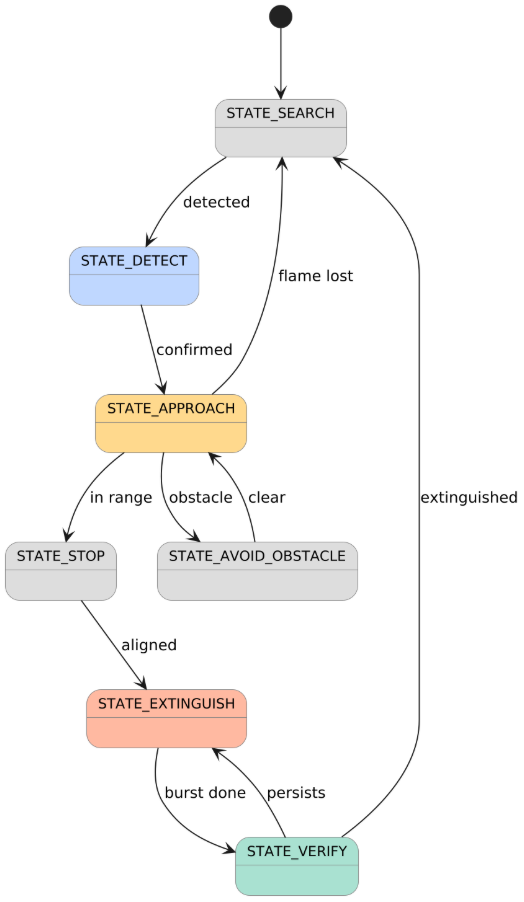
\includegraphics[width=0.55\textwidth]{diagram3.png}
\caption{MOD-07 FSM State Transition Diagram}
\end{figure}

\FloatBarrier
\subsubsection{State Descriptions}

\begin{table}[H]
\centering\small
\begin{tabularx}{\textwidth}{L{3.8cm} L{2.5cm} X}
\toprule
\rowcolor{accent}
\theadtext{State} & \theadtext{Actuators Active} & \theadtext{Description and Exit Condition} \\
\midrule
\rowcolor{white}   \fn{STATE\_SEARCH}         & MOD-04 (rotate)   & Rover rotates in place, polling MOD-02. Exits when \fn{flame\_data\_t.detected == true}. \\[3pt]
\rowcolor{lightbg} \fn{STATE\_DETECT}         & None              & Flame signal confirmed; direction is resolved. Exits immediately to \fn{STATE\_APPROACH} once direction is stable. \\[3pt]
\rowcolor{white}   \fn{STATE\_APPROACH}       & MOD-04 (drive)    & Rover drives toward flame using directional commands. MOD-05 polled every cycle. Exits to \fn{STATE\_STOP} when obstacle is unsafe, to \fn{STATE\_AVOID\_OBSTACLE} on lateral obstacle, or to \fn{STATE\_SEARCH} if flame is lost. \\[3pt]
\rowcolor{lightbg} \fn{STATE\_AVOID\_OBSTACLE} & MOD-04 (steer)  & Rover executes avoidance maneuver. Exits back to \fn{STATE\_APPROACH} when path is clear. \\[3pt]
\rowcolor{white}   \fn{STATE\_STOP}           & None              & All motors halted; rover aligns with flame. Exits to \fn{STATE\_EXTINGUISH}. \\[3pt]
\rowcolor{lightbg} \fn{STATE\_EXTINGUISH}     & MOD-06 (pump on)  & Water pump activated via \fn{suppression\_cmd\_t}. MOD-02 polled for extinction. Exits to \fn{STATE\_VERIFY} after pump burst. \\[3pt]
\rowcolor{white}   \fn{STATE\_VERIFY}         & None              & Confirms \fn{flame\_data\_t.detected == false}. Exits to \fn{STATE\_SEARCH} if flame persists; exits to \fn{STATE\_STOP} (idle) if extinguished. \\
\bottomrule
\end{tabularx}
\caption{FSM state descriptions and exit conditions}
\end{table}

\subsection{Data Types}

\subsubsection{Input Structure}

\begin{lstlisting}[caption={autonomy\_input\_t definition}]
typedef struct {
    flame_data_t flame_data;
    uint16_t     distance_cm;
} autonomy_input_t;
\end{lstlisting}

\begin{table}[H]\centering\small
\begin{tabularx}{\textwidth}{L{3cm} L{3cm} X}
\toprule
\rowcolor{accent}\theadtext{Field} & \theadtext{Type} & \theadtext{Description} \\
\midrule
\rowcolor{white}   \fn{flame\_data}   & \fn{flame\_data\_t} & Flame direction and intensity data from MOD-02 \\
\rowcolor{lightbg} \fn{distance\_cm}  & \fn{uint16\_t}      & Obstacle distance in centimeters from MOD-05 \\
\bottomrule
\end{tabularx}
\caption{Input structure fields}
\end{table}

\subsubsection{Output Structure}

\begin{lstlisting}[caption={autonomy\_output\_t definition}]
typedef struct {
    motion_direction_t motion_cmd;
    uint8_t            speed;
    uint8_t            pump_on;
} autonomy_output_t;
\end{lstlisting}

\begin{table}[H]\centering\small
\begin{tabularx}{\textwidth}{L{3cm} L{3cm} X}
\toprule
\rowcolor{accent}\theadtext{Field} & \theadtext{Type} & \theadtext{Description} \\
\midrule
\rowcolor{white}   \fn{motion\_cmd} & \fn{motion\_direction\_t} & Direction command issued to MOD-04 \\
\rowcolor{lightbg} \fn{speed}       & \fn{uint8\_t}            & PWM speed value (0--255) \\
\rowcolor{white}   \fn{pump\_on}    & \fn{uint8\_t}            & Pump activation flag sent to MOD-06 \\
\bottomrule
\end{tabularx}
\caption{Output structure fields}
\end{table}

\subsection{Public API}

\begin{table}[H]
\centering\small
\begin{tabularx}{\textwidth}{L{5cm} X}
\toprule
\rowcolor{accent}
\theadtext{Function} & \theadtext{Description} \\
\midrule
\rowcolor{white}   \fn{autonomy\_init()}              & Initializes the FSM to \fn{STATE\_SEARCH}. \\
\rowcolor{lightbg} \fn{autonomy\_update(in)}          & Updates FSM with the latest sensor input struct. \\
\rowcolor{white}   \fn{autonomy\_get\_output(out)}    & Returns the current command output struct. \\
\rowcolor{lightbg} \fn{autonomy\_reset()}             & Resets FSM to initial state. \\
\rowcolor{white}   \fn{autonomy\_get\_current\_state()} & Returns the active \fn{autonomy\_state\_t} for telemetry or MOD-08 validation. \\
\bottomrule
\end{tabularx}
\caption{MOD-07 public API}
\end{table}

\subsection{Operational Flow}

\begin{enumerate}[leftmargin=1.5em]
  \item Search for flame by rotating in place.
  \item Detect and confirm flame target; resolve direction.
  \item Move toward flame using directional drive commands.
  \item Avoid obstacles if encountered during approach.
  \item Stop at safe distance from flame.
  \item Activate water pump and begin suppression.
  \item Verify flame extinction via MOD-02.
  \item Return to search mode if flame is still detected.
\end{enumerate}

\subsection{Known Limitations}

\begin{itemize}[leftmargin=1.5em]
  \item No advanced path planning; direct obstacle avoidance is reactive only.
  \item No timeout watchdog for any state; a stuck state loops indefinitely.
  \item No speed ramping; abrupt starts cause wheel slip (see MOD-04 limitations).
  \item Sensor noise from MOD-02 or MOD-05 may cause spurious state transitions.
\end{itemize}


\newpage

% ════════════════════════════════════════════════════════════
%  MOD-08 — INTEGRATION AND TEST MODULE
% ════════════════════════════════════════════════════════════
\section{MOD-08 --- Integration and Test Module}

\subsection{Module Purpose}

MOD-08 serves as the system-wide validation and quality assurance layer for the
Autonomous Fire Detection and Suppression Rover. Its primary responsibility is to
verify that all eight modules operate correctly both individually and in concert
before and during field deployment.

The module provides two complementary testing modes: a \textbf{real hardware
self-check} that exercises every physical peripheral on the rover, and a
\textbf{simulation mode} that injects synthetic sensor data into the system,
allowing full Finite State Machine (FSM) validation without requiring a physical
fire source or any hardware.

\subsection{Dependencies}

\begin{table}[H]
\centering\small
\begin{tabularx}{\textwidth}{L{4.5cm} L{2.5cm} X}
\toprule
\rowcolor{accent}
\theadtext{Module Name} & \theadtext{ID} & \theadtext{Usage in MOD-08} \\
\midrule
\rowcolor{white}   Flame Sensing HW    & \fn{MOD-01} & Sensor presence validation during self-check \\
\rowcolor{lightbg} Flame Detection SW  & \fn{MOD-02} & Full detection pipeline verification via \fn{flame\_data\_t} \\
\rowcolor{white}   Locomotion HW       & \fn{MOD-03} & Motor driver response test \\
\rowcolor{lightbg} Motion Control SW   & \fn{MOD-04} & Movement command verification via \fn{motion\_direction\_t} \\
\rowcolor{white}   Distance Sensing    & \fn{MOD-05} & Ultrasonic obstacle detection validation \\
\rowcolor{lightbg} Fire Suppression HW & \fn{MOD-06} & Relay and pump activation test \\
\rowcolor{white}   Autonomy SW         & \fn{MOD-07} & End-to-end FSM behavior testing with injected triggers \\
\bottomrule
\end{tabularx}
\caption{MOD-08 dependencies}
\end{table}

\subsection{Public API}

\subsubsection{Public Functions}

\begin{table}[H]
\centering\small
\begin{tabularx}{\textwidth}{L{4.5cm} L{4cm} L{2.5cm} X}
\toprule
\rowcolor{accent}
\theadtext{Function} & \theadtext{Parameters} & \theadtext{Return} & \theadtext{Description} \\
\midrule
\rowcolor{white}   \fn{test\_init()}                  & \fn{void}                               & \fn{void}            & Initialises internal state and links to all dependent modules. \\
\rowcolor{lightbg} \fn{test\_set\_mode()}             & \fn{test\_mode\_t mode}                 & \fn{void}            & Switches between \fn{TEST\_MODE\_REAL} and \fn{TEST\_MODE\_SIMULATION}. \\
\rowcolor{white}   \fn{test\_run\_self\_check()}      & \fn{void}                               & \fn{test\_status\_t} & Sequentially validates all hardware peripherals; returns first failure code or \fn{TEST\_OK}. \\
\rowcolor{lightbg} \fn{test\_get\_report()}           & \fn{test\_report\_t *report}            & \fn{void}            & Fills caller-owned struct with per-subsystem pass/fail flags. \\
\rowcolor{white}   \fn{test\_set\_simulation\_data()} & \fn{const test\_simulation\_input\_t *data} & \fn{void}        & Injects synthetic flame and distance data for simulation runs. \\
\rowcolor{lightbg} \fn{test\_update()}                & \fn{void}                               & \fn{void}            & Periodic monitoring tick; logs anomalies during continuous operation. \\
\bottomrule
\end{tabularx}
\caption{MOD-08 public functions}
\end{table}

\subsubsection{Data Types}

\begin{table}[H]
\centering\small
\begin{tabularx}{\textwidth}{L{4.5cm} L{2cm} X}
\toprule
\rowcolor{accent}
\theadtext{Type} & \theadtext{Kind} & \theadtext{Fields / Values} \\
\midrule
\rowcolor{white}   \fn{test\_status\_t}            & enum   & \fn{TEST\_OK}, \fn{TEST\_FAIL\_SENSOR}, \fn{TEST\_FAIL\_DISTANCE}, \fn{TEST\_FAIL\_MOTOR}, \fn{TEST\_FAIL\_PUMP} \\
\rowcolor{lightbg} \fn{test\_mode\_t}              & enum   & \fn{TEST\_MODE\_REAL}, \fn{TEST\_MODE\_SIMULATION} \\
\rowcolor{white}   \fn{test\_report\_t}            & struct & \fn{sensor\_ok}, \fn{distance\_ok}, \fn{motor\_ok}, \fn{pump\_ok} (all \fn{int}) \\
\rowcolor{lightbg} \fn{test\_simulation\_input\_t} & struct & \fn{flame\_data} (\fn{flame\_data\_t} from MOD-02), \fn{distance\_cm} (\fn{uint16\_t}) \\
\bottomrule
\end{tabularx}
\caption{MOD-08 data types}
\end{table}

\subsection{Module Connections}

MOD-08 occupies a unique position in the architecture: it has \textbf{read access
to every module's output} for validation purposes, and \textbf{write/inject access}
to MOD-02, MOD-05, and MOD-07 for simulation. In production mode it is passive;
in test mode it becomes the data source.

\begin{table}[H]
\centering\small
\begin{tabularx}{\textwidth}{L{2cm} L{2cm} L{4cm} L{2.5cm} X}
\toprule
\rowcolor{accent}
\theadtext{From} & \theadtext{To} & \theadtext{Signal / Data} & \theadtext{Direction} & \theadtext{Notes} \\
\midrule
\rowcolor{white}   \fn{MOD-08} & \fn{MOD-02} & \fn{simulate\_flame}    & 08 $\rightarrow$ 02 & Injected \fn{flame\_data\_t} for simulation runs \\
\rowcolor{lightbg} \fn{MOD-08} & \fn{MOD-05} & \fn{simulate\_distance} & 08 $\rightarrow$ 05 & Injected \fn{distance\_cm} for simulation runs \\
\rowcolor{white}   \fn{MOD-08} & \fn{MOD-07} & \fn{test\_triggers}     & 08 $\rightarrow$ 07 & FSM state injection for behavioral testing \\
\rowcolor{lightbg} \fn{MOD-01} & \fn{MOD-08} & \fn{sensor\_status}     & 01 $\rightarrow$ 08 & Sensor presence confirmed during self-check \\
\rowcolor{white}   \fn{MOD-03} & \fn{MOD-08} & \fn{motor\_status}      & 03 $\rightarrow$ 08 & Motor driver response during self-check \\
\rowcolor{lightbg} \fn{MOD-05} & \fn{MOD-08} & \fn{dist\_reading}      & 05 $\rightarrow$ 08 & Ultrasonic ping result for validation \\
\rowcolor{white}   \fn{MOD-06} & \fn{MOD-08} & \fn{pump\_status}       & 06 $\rightarrow$ 08 & Relay activation confirmation \\
\rowcolor{lightbg} \fn{MOD-07} & \fn{MOD-08} & \fn{fsm\_state}         & 07 $\rightarrow$ 08 & Current FSM state read for behavioral validation \\
\bottomrule
\end{tabularx}
\caption{MOD-08 inter-module signal map}
\end{table}


\subsection{Operational Flow}

\begin{table}[H]
\centering\small
\begin{tabularx}{\textwidth}{C{0.7cm} L{7cm} X}
\toprule
\rowcolor{accent}
\theadtext{\#} & \theadtext{Real Mode} & \theadtext{Simulation Mode} \\
\midrule
\rowcolor{white}   1 & \fn{test\_init()} --- link all modules & \fn{test\_init()} --- link all modules \\
\rowcolor{lightbg} 2 & \fn{test\_set\_mode(TEST\_MODE\_REAL)} & \fn{test\_set\_mode(TEST\_MODE\_SIMULATION)} \\
\rowcolor{white}   3 & \fn{test\_run\_self\_check()} --- ping each peripheral & \fn{test\_set\_simulation\_data()} --- load scenario \\
\rowcolor{lightbg} 4 & \fn{test\_get\_report()} --- read pass/fail flags & \fn{test\_update()} --- inject data into MOD-02/05/07 \\
\rowcolor{white}   5 & \fn{test\_update()} --- continuous monitoring loop & Read \fn{autonomy\_get\_current\_state()} to assert \\
\bottomrule
\end{tabularx}
\caption{MOD-08 operational flows}
\end{table}

\subsection{Known Limitations and TODOs}

\subsubsection{Current Limitations}

\begin{itemize}[leftmargin=1.5em]
  \item Test routines depend on controlled environment conditions; field noise may produce false failures.
  \item Simulation scenarios are limited to a single static input snapshot; dynamic sequences are not yet supported.
  \item No detailed per-component error logging; \fn{test\_report\_t} provides only binary pass/fail per subsystem.
  \item \fn{test\_update()} does not yet implement continuous flame-loss or motor-stall detection.
\end{itemize}

\subsubsection{Planned Improvements}

\begin{itemize}[leftmargin=1.5em]
  \item[$\square$] Add granular error codes to \fn{test\_report\_t} (e.g., which sensor index failed).
  \item[$\square$] Extend simulation to support multi-step scenarios with changing distance and flame direction over time.
  \item[$\square$] Implement automated test logging to serial output or SD card for field debugging.
  \item[$\square$] Integrate continuous system monitoring with alert thresholds in \fn{test\_update()}.
  \item[$\square$] Add a dedicated stress-test mode that cycles \fn{STATE\_EXTINGUISH} repeatedly to validate relay cooldown (MOD-06).
\end{itemize}


\vfill
{\color{accent}\rule{\linewidth}{1.5pt}}
\begin{center}
  \small
  CSE 396 Group 2 \quad---\quad Assignment 3: Module Documentation \quad---\quad April 2026
\end{center}

\end{document}
